%%%%%%%%%%%%%%%%%%%%%%%%%%%%%%%%%%%%%%%%%
% Short Sectioned Assignment
% LaTeX Template
% Version 1.0 (5/5/12)
%
% This template has been downloaded from:
% http://www.LaTeXTemplates.com
%
% Original author:
% Frits Wenneker (http://www.howtotex.com)
%
% License:
% CC BY-NC-SA 3.0 (http://creativecommons.org/licenses/by-nc-sa/3.0/)
%
%%%%%%%%%%%%%%%%%%%%%%%%%%%%%%%%%%%%%%%%%

%----------------------------------------------------------------------------------------
%	PACKAGES AND OTHER DOCUMENT CONFIGURATIONS
%----------------------------------------------------------------------------------------

\documentclass[paper=a4, fontsize=11pt]{scrartcl} % A4 paper and 11pt font size

\usepackage[T1]{fontenc} % Use 8-bit encoding that has 256 glyphs
\usepackage{fourier} % Use the Adobe Utopia font for the document - comment this line to return to the LaTeX default
\usepackage[english]{babel} % English language/hyphenation
\usepackage{amsmath,amsfonts,amsthm} % Math packages

\usepackage{lipsum} % Used for inserting dummy 'Lorem ipsum' text into the template

\usepackage{sectsty} % Allows customizing section commands
\usepackage{graphicx}
\allsectionsfont{\centering \normalfont\scshape} % Make all sections centered, the default font and small caps

\usepackage{fancyhdr} % Custom headers and footers
\pagestyle{fancyplain} % Makes all pages in the document conform to the custom headers and footers
\fancyhead{} % No page header - if you want one, create it in the same way as the footers below
\fancyfoot[L]{} % Empty left footer
\fancyfoot[C]{} % Empty center footer
\fancyfoot[R]{\thepage} % Page numbering for right footer
\renewcommand{\headrulewidth}{0pt} % Remove header underlines
\renewcommand{\footrulewidth}{0pt} % Remove footer underlines
\setlength{\headheight}{13.6pt} % Customize the height of the header

\numberwithin{equation}{section} % Number equations within sections (i.e. 1.1, 1.2, 2.1, 2.2 instead of 1, 2, 3, 4)
\numberwithin{figure}{section} % Number figures within sections (i.e. 1.1, 1.2, 2.1, 2.2 instead of 1, 2, 3, 4)
\numberwithin{table}{section} % Number tables within sections (i.e. 1.1, 1.2, 2.1, 2.2 instead of 1, 2, 3, 4)

\setlength\parindent{0pt} % Removes all indentation from paragraphs - comment this line for an assignment with lots of text

\usepackage[T1]{fontenc}
\usepackage[utf8]{inputenc}
%----------------------------------------------------------------------------------------
%	TITLE SECTION
%----------------------------------------------------------------------------------------

\newcommand{\horrule}[1]{\rule{\linewidth}{#1}} % Create horizontal rule command with 1 argument of height

\title{}
\title{	
\normalfont \normalsize 
\textsc{Ecole Nationale des Ingénieurs de Brest} \\ [25pt] % Your university, school and/or department name(s)
\horrule{0.5pt} \\[0.4cm] % Thin top horizontal rule
\huge Modèle de Markov Caché pour la prise de décision de robots ou d'entités virtuelles \\ % The assignment title
\horrule{2pt} \\[0.5cm] % Thick bottom horizontal rule
}

\author{Arthur Le Guennec \and Kwon-Young Choi}

\date{\normalsize\today} % Today's date or a custom date

\begin{document}

\maketitle % Print the title

%----------------------------------------------------------------------------------------
%	PROBLEM 1
%----------------------------------------------------------------------------------------

\section{Principe général des Modèles de Markov Caché}

Un HMM (Hidden Markov Model en anglais ou Modèle de Markov Caché en français) est une modélisation stochastique d'un automate avec des états cachés (notés Ht) et des états observables (notés St).
Les états cachés sont modélisés par un chaîne de Markov.
L'utilisation d'une chaine de Markov induit que le modèle est discret dans le temps et peut aussi être discret dans ses états.
Les chaine de Markov possède la propriété de Markov, ce qui implique que la probabilité d'être dans un état Ht+1 ne dépend pas de tous les états précédents.
Chacun des états du HMM a donc une probabilité de transition vers les autres états.
Les état observables ne dépendent que de l'état courant.

\begin{figure}[bp]
  \centering
  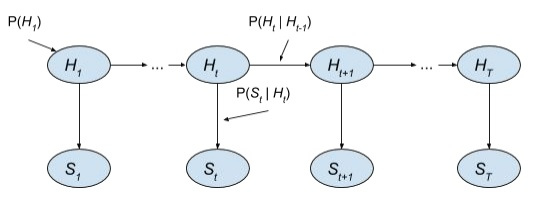
\includegraphics[scale=0.9]{hmm}
  \caption{\label{hmm} Modélisation d'un Modèle de Markov Caché.}
\end{figure}

Les HMM sont beaucoup utilisés dans  la reconnaissance de forme, comme la reconnaissance des gestes, ou la reconnaissance vocale.

\section{HMM utilisé pour la prise de décision}

Un modèle de markov caché utilisé pour la prise de décision est le POMDP (Partially Observable Markov Decision Process ou processus de décision markovien partiellement observable).
Ce modèle dérive de MDP (Markov Decision Process ou processus de décision markovienne) qui est un modèle particulier des chaînes de markov.
À la différence des autres chaînes de markov, les MDP permettent à un agent d'influencer le système.
L'état suivant dépend donc de l'état actuel et de l'action actuelle.
L'effet de l'action sur l'état suivant n'est cependant pas connue.
On a donc une incertitude sur l'effet de l'action, comme pour un MDP, mais on a aussi une autre incertitude sur l'état dans lequel on se trouve.

Concernant la prise de décision, les HMM peuvent être utilisés dans des domaines où toutes les variables ne sont pas connues.
Par exemple, dans un jeu de poker, les cartes des adversaires ne sont pas connus par le joueur.
Le modèle POMDP pourrait permettre de choisir la meilleur stratégie à appliquer selon le mode de jeu des adversaires.
Nous allons par la suite voir une autre application des POMDP utilisé dans le cadre de la navigation d'un robot dans environnement de bureau.

\section{Architecture de navigation de robot en utilisant les POMDP}

Dans l'article \cite{koenig_xavier_1998}, les auteurs ont voulu modéliser une architecture de navigation robotique en utilisant un processus de décision markovien partiellement observable (POMDP).
Le but de l'article est construire un robot capable d'effectuer des livraisons dans un environnement de bureau de travail.
Cela implique que le robot aura à se déplacer dans des corridors ou des salles avec des portes closes ou ouvertes et cela pendant de longues périodes de temps.

Pour pouvoir construire une architecture de navigation capable de réaliser de telles tâches, cela implique que le robot devra pouvoir faire face à toutes sortes d'incertitudes comme la longueur des corridors, l'état d'une porte: fermée ou ouverte, \ldots
C'est dans cette optique de modéliser l'incertitude que les auteurs ont choisis d'utiliser des POMDP.
En effet, ce modèle permet de modéliser explicitement toutes sortes d'incertitude:
\begin{itemize}
  \item incertitude de positionnement
  \item incertitude des capteurs et des données capteurs
  \item incertitude de la position initiale
  \item incertitude de l'environnement (longueur des corridors, portes fermées, \ldots)
\end{itemize}
La force d'un POMDP est le fait qu'il n'utilise pas une seule estimation de la position du robot, mais utilise une distribution de probabilité entière pour modéliser sa position.
Cela implique que le robot ne sait jamais précisément où il se trouve.
Cependant, cela veut aussi que le robot n'est jamais complètement perdu et a toujours une croyance de sa position actuelle.
Cette croyance est mise à jour régulièrement par les informations de capteurs comme des capteurs de distances parcourus ou des capteurs de présence.
Toutes ces propriétés des POMDP permet de modéliser une architecture de navigation robuste de robot pour une utilisation de tout les jours.

D'autre part, le POMDP est directement généré à partir de la carte topologique de l'environnement (et des variations possibles de l'environnement) et des modèles de ses capteurs et de ses actionneurs.
L'utilisation concrète des POMDP a donc permis:
\begin{itemize}
  \item d'estimer de la position du robot
  \item une planification de la trajectoire: où, quand, comment
  \item de contrôler la navigation
  \item l'apprentissage et l'amélioration constante du modèle
\end{itemize}


\bibliographystyle{plain}
\bibliography{hmm}

%\section{Problem title}

%\lipsum[2] % Dummy text

%\begin{align} 
%\begin{split}
%(x+y)^3 	&= (x+y)^2(x+y)\\
%&=(x^2+2xy+y^2)(x+y)\\
%&=(x^3+2x^2y+xy^2) + (x^2y+2xy^2+y^3)\\
%&=x^3+3x^2y+3xy^2+y^3
%\end{split}					
%\end{align}

%Phasellus viverra nulla ut metus varius laoreet. Quisque rutrum. Aenean imperdiet. Etiam ultricies nisi vel augue. Curabitur ullamcorper ultricies

%%------------------------------------------------

%\subsection{Heading on level 2 (subsection)}

%Lorem ipsum dolor sit amet, consectetuer adipiscing elit. 
%\begin{align}
%A = 
%\begin{bmatrix}
%A_{11} & A_{21} \\
%A_{21} & A_{22}
%\end{bmatrix}
%\end{align}
%Aenean commodo ligula eget dolor. Aenean massa. Cum sociis natoque penatibus et magnis dis parturient montes, nascetur ridiculus mus. Donec quam felis, ultricies nec, pellentesque eu, pretium quis, sem.

%%------------------------------------------------

%\subsubsection{Heading on level 3 (subsubsection)}

%\lipsum[3] % Dummy text

%\paragraph{Heading on level 4 (paragraph)}

%\lipsum[6] % Dummy text

%%----------------------------------------------------------------------------------------
%%	PROBLEM 2
%%----------------------------------------------------------------------------------------

%\section{Lists}

%%------------------------------------------------

%\subsection{Example of list (3*itemize)}
%\begin{itemize}
	%\item First item in a list 
		%\begin{itemize}
		%\item First item in a list 
			%\begin{itemize}
			%\item First item in a list 
			%\item Second item in a list 
			%\end{itemize}
		%\item Second item in a list 
		%\end{itemize}
	%\item Second item in a list 
%\end{itemize}

%%------------------------------------------------

%\subsection{Example of list (enumerate)}
%\begin{enumerate}
%\item First item in a list 
%\item Second item in a list 
%\item Third item in a list
%\end{enumerate}

%----------------------------------------------------------------------------------------

\end{document}
